\chapter{شاره‌ها و برش‌ها}

در این فصل، روی دو مسئله زیر تمرکز می‌کنیم:

\begin{itemize}
\item \key{یافتن بیشینه شاره}:
بیشترین مقدار شاره که می‌توان از یک رأس به رأس دیگر فرستاد چقدر است؟
\item \key{یافتن کمینه برش}:
مجموعه‌ای از یال‌ها با کمینه وزن که دو رأس گراف را از هم جدا کند چیست؟
\end{itemize}

ورودی هر دو مسئله یک گراف جهت‌دار و وزن‌دار شامل دو رأس خاص است:
\emph{مبدأ} رأسی بدون یال ورودی است،
و \emph{مقصد} رأسی بدون یال خروجی است.

به عنوان مثال، از گراف زیر استفاده می‌کنیم
که رأس 1 مبدأ و رأس 6
مقصد است:

\begin{center}
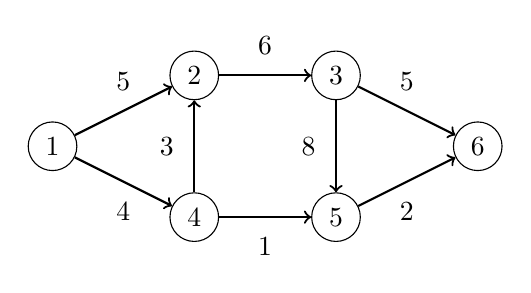
\begin{tikzpicture}[scale=0.9]
\node[draw, circle] (1) at (1,2) {$1$};
\node[draw, circle] (2) at (3,3) {$2$};
\node[draw, circle] (3) at (5,3) {$3$};
\node[draw, circle] (4) at (7,2) {$6$};
\node[draw, circle] (5) at (3,1) {$4$};
\node[draw, circle] (6) at (5,1) {$5$};
\path[draw,thick,->] (1) -- node[font=\small,label=5] {} (2);
\path[draw,thick,->] (2) -- node[font=\small,label=6] {} (3);
\path[draw,thick,->] (3) -- node[font=\small,label=5] {} (4);
\path[draw,thick,->] (1) -- node[font=\small,label=below:4] {} (5);
\path[draw,thick,->] (5) -- node[font=\small,label=below:1] {} (6);
\path[draw,thick,->] (6) -- node[font=\small,label=below:2] {} (4);
\path[draw,thick,<-] (2) -- node[font=\small,label=left:3] {} (5);
\path[draw,thick,->] (3) -- node[font=\small,label=left:8] {} (6);
\end{tikzpicture}
\end{center}

\subsubsection{بیشینه شاره}

\index{شاره}
\index{بیشینه شاره}

در مسئله \key{بیشینه شاره}،
هدف فرستادن بیشترین مقدار ممکن شاره
از مبدأ به مقصد است.
وزن هر یال ظرفیتی است که
شاره عبوری از آن یال را محدود می‌کند.
در هر رأس میانی،
مقدار شاره ورودی و خروجی
باید برابر باشد.

برای نمونه، بیشینه مقدار شاره
در گراف مثال برابر 7 است.
تصویر زیر نحوه هدایت شاره را نشان می‌دهد:

\begin{center}
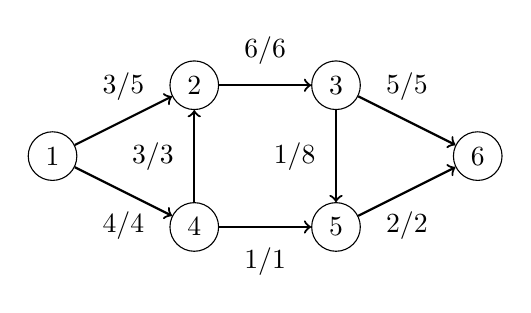
\begin{tikzpicture}[scale=0.9]
\node[draw, circle] (1) at (1,2) {$1$};
\node[draw, circle] (2) at (3,3) {$2$};
\node[draw, circle] (3) at (5,3) {$3$};
\node[draw, circle] (4) at (7,2) {$6$};
\node[draw, circle] (5) at (3,1) {$4$};
\node[draw, circle] (6) at (5,1) {$5$};
\path[draw,thick,->] (1) -- node[font=\small,label=3/5] {} (2);
\path[draw,thick,->] (2) -- node[font=\small,label=6/6] {} (3);
\path[draw,thick,->] (3) -- node[font=\small,label=5/5] {} (4);
\path[draw,thick,->] (1) -- node[font=\small,label=below:4/4] {} (5);
\path[draw,thick,->] (5) -- node[font=\small,label=below:1/1] {} (6);
\path[draw,thick,->] (6) -- node[font=\small,label=below:2/2] {} (4);
\path[draw,thick,<-] (2) -- node[font=\small,label=left:3/3] {} (5);
\path[draw,thick,->] (3) -- node[font=\small,label=left:1/8] {} (6);
\end{tikzpicture}
\end{center}

نمادگذاری $v/k$ به این معنی است
که جریانی به اندازه $v$ واحد از
یالی با ظرفیت $k$ واحد عبور داده شده است.
اندازه جریان $7$ است،
زیرا مبدأ $3+4$ واحد جریان می‌فرستد
و مقصد $5+2$ واحد جریان دریافت می‌کند.
به‌سادگی می‌توان دریافت که این جریان بیشینه است،
زیرا ظرفیت کل یال‌های
منتهی به مقصد برابر $7$ است.

\subsubsection{برش کمینه}

\index{cut}
\index{minimum cut}

در مسئله \key{برش کمینه} (minimum cut)،
هدف ما حذف مجموعه‌ای
از یال‌ها از گراف است
به‌طوری که پس از حذف هیچ مسیری از مبدأ
به مقصد وجود نداشته باشد
و مجموع وزن یال‌های حذف‌شده
کمینه باشد.

اندازه کمینه برش در گراف نمونه برابر 7 است.
کافی است یال‌های $2 \rightarrow 3$
و $4 \rightarrow 5$ را حذف کنیم:

\begin{center}
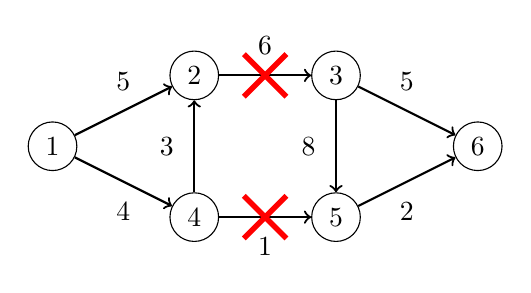
\begin{tikzpicture}[scale=0.9]
\node[draw, circle] (1) at (1,2) {$1$};
\node[draw, circle] (2) at (3,3) {$2$};
\node[draw, circle] (3) at (5,3) {$3$};
\node[draw, circle] (4) at (7,2) {$6$};
\node[draw, circle] (5) at (3,1) {$4$};
\node[draw, circle] (6) at (5,1) {$5$};
\path[draw,thick,->] (1) -- node[font=\small,label=5] {} (2);
\path[draw,thick,->] (2) -- node[font=\small,label=6] {} (3);
\path[draw,thick,->] (3) -- node[font=\small,label=5] {} (4);
\path[draw,thick,->] (1) -- node[font=\small,label=below:4] {} (5);
\path[draw,thick,->] (5) -- node[font=\small,label=below:1] {} (6);
\path[draw,thick,->] (6) -- node[font=\small,label=below:2] {} (4);
\path[draw,thick,<-] (2) -- node[font=\small,label=left:3] {} (5);
\path[draw,thick,->] (3) -- node[font=\small,label=left:8] {} (6);

\path[draw=red,thick,-,line width=2pt] (4-.3,3-.3) -- (4+.3,3+.3);
\path[draw=red,thick,-,line width=2pt] (4-.3,3+.3) -- (4+.3,3-.3);
\path[draw=red,thick,-,line width=2pt] (4-.3,1-.3) -- (4+.3,1+.3);
\path[draw=red,thick,-,line width=2pt] (4-.3,1+.3) -- (4+.3,1-.3);
\end{tikzpicture}
\end{center}

پس از حذف این یال‌ها،
هیچ مسیری از مبدأ به مقصد وجود نخواهد داشت.
اندازه برش برابر $7$ است،
زیرا وزن‌های یال‌های حذف‌شده
$6$ و $1$ هستند.
این برش کمینه است، زیرا هیچ روش
معتبری برای حذف یال‌ها از گراف وجود ندارد به شکلی که
مجموع وزن آن‌ها کمتر از $7$ شود.
\\\\
تصادفی نیست که
اندازه بیشینه یک جریان
و اندازه کمینه یک برش
در مثال بالا یکسان است.
مشخص می‌شود که یک جریان بیشینه
و یک برش کمینه
\emph{همیشه} هم‌اندازه‌اند؛
بنابراین این مفاهیم دو روی یک سکه‌اند.

در ادامه الگوریتم فورد–فالکرسون
را بررسی می‌کنیم که می‌توان از آن برای یافتن
جریان بیشینه و برش کمینه در یک گراف استفاده کرد.
این الگوریتم همچنین به ما کمک می‌کند تا بفهمیم
\emph{چرا} این دو مقدار همواره برابر هستند.

\section{الگوریتم فورد–فالکرسون}

\index{Ford–Fulkerson algorithm}

\key{الگوریتم فورد–فالکرسون} \cite{for56}
جریان بیشینه را در یک گراف می‌یابد.
الگوریتم با جریان تهی آغاز می‌شود،
و در هر گام مسیری از مبدأ
به مقصد پیدا می‌کند که جریان بیشتری تولید می‌نماید.
در نهایت، هنگامی که الگوریتم نتواند جریان را بیش از این
افزایش دهد، جریان بیشینه یافته شده است.

این الگوریتم از نمایش ویژه‌ای از گراف استفاده می‌کند که در آن هر یال اصلی یک یال معکوس در جهت مخالف دارد.
وزن هر یال نشان می‌دهد چه مقدار شار دیگر می‌توان از آن عبور داد.
در آغاز الگوریتم، وزن هر یال اصلی برابر با ظرفیت آن یال
و وزن هر یال معکوس برابر با صفر است.

\begin{samepage}
نمایش جدید برای گراف نمونه به شکل زیر است:

\begin{center}
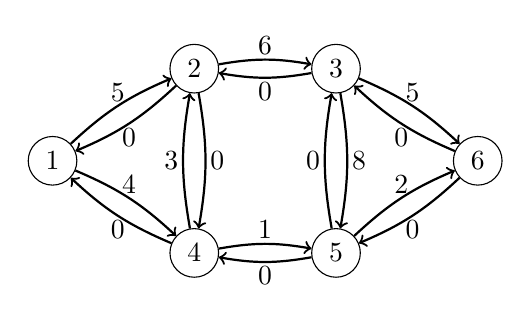
\begin{tikzpicture}[scale=0.9,label distance=-2mm]
\node[draw, circle] (1) at (1,1.3) {$1$};
\node[draw, circle] (2) at (3,2.6) {$2$};
\node[draw, circle] (3) at (5,2.6) {$3$};
\node[draw, circle] (4) at (7,1.3) {$6$};
\node[draw, circle] (5) at (3,0) {$4$};
\node[draw, circle] (6) at (5,0) {$5$};

\path[draw,thick,->] (1) edge [bend left=10] node[font=\small,label=5] {} (2);
\path[draw,thick,->] (2) edge [bend left=10] node[font=\small,label=below:0] {} (1);
\path[draw,thick,->] (2) edge [bend left=10] node[font=\small,label=6] {} (3);
\path[draw,thick,->] (3) edge [bend left=10] node[font=\small,label=below:0] {} (2);
\path[draw,thick,->] (3) edge [bend left=10] node[font=\small,label=5] {} (4);
\path[draw,thick,->] (4) edge [bend left=10] node[font=\small,label=below:0] {} (3);
\path[draw,thick,->] (1) edge [bend left=10] node[font=\small,label=4] {} (5);
\path[draw,thick,->] (5) edge [bend left=10] node[font=\small,label=below:0] {} (1);
\path[draw,thick,->] (5) edge [bend left=10] node[font=\small,label=1] {} (6);
\path[draw,thick,->] (6) edge [bend left=10] node[font=\small,label=below:0] {} (5);
\path[draw,thick,->] (6) edge [bend left=10] node[font=\small,label=2] {} (4);
\path[draw,thick,->] (4) edge [bend left=10] node[font=\small,label=below:0] {} (6);
\path[draw,thick,->] (5) edge [bend left=10] node[font=\small,label=left:3] {} (2);
\path[draw,thick,->] (2) edge [bend left=10] node[font=\small,label=right:0] {} (5);
\path[draw,thick,->] (3) edge [bend left=10] node[font=\small,label=right:8] {} (6);
\path[draw,thick,->] (6) edge [bend left=10] node[font=\small,label=left:0] {} (3);
\end{tikzpicture}
\end{center}
\end{samepage}

\subsubsection{توصیف الگوریتم}

الگوریتم فورد-فالکرسون از چندین مرحله تشکیل شده است.
در هر مرحله، الگوریتم مسیری از مبدأ به مقصد پیدا می‌کند
به طوری که هر یال در این مسیر دارای وزنی مثبت باشد.
اگر بیش از یک مسیر ممکن وجود داشته باشد،
می‌توانیم هر یک از آنها را انتخاب کنیم.

برای مثال، فرض کنید مسیر زیر را انتخاب کنیم:

\begin{center}
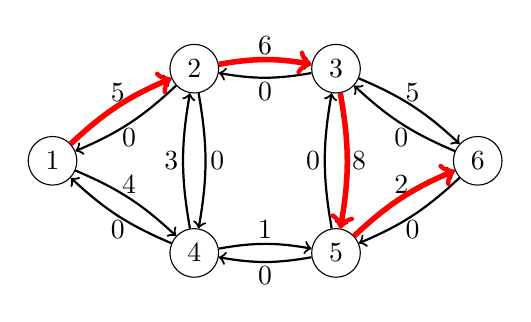
\begin{tikzpicture}[scale=0.9,label distance=-2mm]
\node[draw, circle] (1) at (1,1.3) {$1$};
\node[draw, circle] (2) at (3,2.6) {$2$};
\node[draw, circle] (3) at (5,2.6) {$3$};
\node[draw, circle] (4) at (7,1.3) {$6$};
\node[draw, circle] (5) at (3,0) {$4$};
\node[draw, circle] (6) at (5,0) {$5$};

\path[draw,thick,->] (1) edge [bend left=10] node[font=\small,label=5] {} (2);
\path[draw,thick,->] (2) edge [bend left=10] node[font=\small,label=below:0] {} (1);
\path[draw,thick,->] (2) edge [bend left=10] node[font=\small,label=6] {} (3);
\path[draw,thick,->] (3) edge [bend left=10] node[font=\small,label=below:0] {} (2);
\path[draw,thick,->] (3) edge [bend left=10] node[font=\small,label=5] {} (4);
\path[draw,thick,->] (4) edge [bend left=10] node[font=\small,label=below:0] {} (3);
\path[draw,thick,->] (1) edge [bend left=10] node[font=\small,label=4] {} (5);
\path[draw,thick,->] (5) edge [bend left=10] node[font=\small,label=below:0] {} (1);
\path[draw,thick,->] (5) edge [bend left=10] node[font=\small,label=1] {} (6);
\path[draw,thick,->] (6) edge [bend left=10] node[font=\small,label=below:0] {} (5);
\path[draw,thick,->] (6) edge [bend left=10] node[font=\small,label=2] {} (4);
\path[draw,thick,->] (4) edge [bend left=10] node[font=\small,label=below:0] {} (6);
\path[draw,thick,->] (5) edge [bend left=10] node[font=\small,label=left:3] {} (2);
\path[draw,thick,->] (2) edge [bend left=10] node[font=\small,label=right:0] {} (5);
\path[draw,thick,->] (3) edge [bend left=10] node[font=\small,label=right:8] {} (6);
\path[draw,thick,->] (6) edge [bend left=10] node[font=\small,label=left:0] {} (3);

\path[draw=red,thick,->,line width=2pt] (1) edge [bend left=10] (2);
\path[draw=red,thick,->,line width=2pt] (2) edge [bend left=10] (3);
\path[draw=red,thick,->,line width=2pt] (3) edge [bend left=10] (6);
\path[draw=red,thick,->,line width=2pt] (6) edge [bend left=10] (4);
\end{tikzpicture}
\end{center}

پس از انتخاب مسیر، شار به اندازهٔ $x$ واحد افزایش می‌یابد
که در آن $x$ کمترین وزن یال روی مسیر است.
علاوه بر این، وزن هر یال روی مسیر
به اندازهٔ $x$ کاهش و وزن هر یال معکوس
به اندازهٔ $x$ افزایش می‌یابد.

در مسیر بالا، وزن یال‌ها
برابر ۵، ۶، ۸ و ۲ است.
کمترین وزن ۲ است،
بنابراین شار به اندازهٔ ۲ افزایش می‌یابد
و گراف جدید به شکل زیر خواهد بود:

\begin{center}
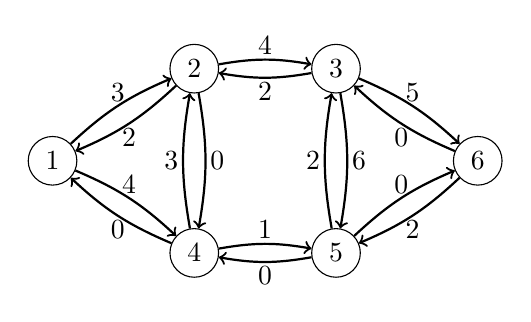
\begin{tikzpicture}[scale=0.9,label distance=-2mm]
\node[draw, circle] (1) at (1,1.3) {$1$};
\node[draw, circle] (2) at (3,2.6) {$2$};
\node[draw, circle] (3) at (5,2.6) {$3$};
\node[draw, circle] (4) at (7,1.3) {$6$};
\node[draw, circle] (5) at (3,0) {$4$};
\node[draw, circle] (6) at (5,0) {$5$};

\path[draw,thick,->] (1) edge [bend left=10] node[font=\small,label=3] {} (2);
\path[draw,thick,->] (2) edge [bend left=10] node[font=\small,label=below:2] {} (1);
\path[draw,thick,->] (2) edge [bend left=10] node[font=\small,label=4] {} (3);
\path[draw,thick,->] (3) edge [bend left=10] node[font=\small,label=below:2] {} (2);
\path[draw,thick,->] (3) edge [bend left=10] node[font=\small,label=5] {} (4);
\path[draw,thick,->] (4) edge [bend left=10] node[font=\small,label=below:0] {} (3);
\path[draw,thick,->] (1) edge [bend left=10] node[font=\small,label=4] {} (5);
\path[draw,thick,->] (5) edge [bend left=10] node[font=\small,label=below:0] {} (1);
\path[draw,thick,->] (5) edge [bend left=10] node[font=\small,label=1] {} (6);
\path[draw,thick,->] (6) edge [bend left=10] node[font=\small,label=below:0] {} (5);
\path[draw,thick,->] (6) edge [bend left=10] node[font=\small,label=0] {} (4);
\path[draw,thick,->] (4) edge [bend left=10] node[font=\small,label=below:2] {} (6);
\path[draw,thick,->] (5) edge [bend left=10] node[font=\small,label=left:3] {} (2);
\path[draw,thick,->] (2) edge [bend left=10] node[font=\small,label=right:0] {} (5);
\path[draw,thick,->] (3) edge [bend left=10] node[font=\small,label=right:6] {} (6);
\path[draw,thick,->] (6) edge [bend left=10] node[font=\small,label=left:2] {} (3);
\end{tikzpicture}
\end{center}

ایده این است که افزایش شار، مقدار شاری را که می‌تواند در آینده از یال‌ها عبور کند کاهش می‌دهد.
از سوی دیگر، می‌توان بعداً با استفاده از یال‌های معکوس گراف، شار را لغو کرد اگر مشخص شود که هدایت شار از مسیری دیگر سودمندتر است.

الگوریتم تا زمانی که مسیری با یال‌های دارای وزن مثبت از مبدأ به مقصد وجود داشته باشد، شار را افزایش می‌دهد.
در این مثال، مسیر بعدی می‌تواند به صورت زیر باشد:

\begin{center}
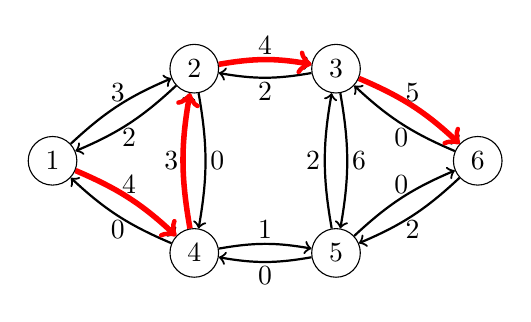
\begin{tikzpicture}[scale=0.9,label distance=-2mm]
\node[draw, circle] (1) at (1,1.3) {$1$};
\node[draw, circle] (2) at (3,2.6) {$2$};
\node[draw, circle] (3) at (5,2.6) {$3$};
\node[draw, circle] (4) at (7,1.3) {$6$};
\node[draw, circle] (5) at (3,0) {$4$};
\node[draw, circle] (6) at (5,0) {$5$};

\path[draw,thick,->] (1) edge [bend left=10] node[font=\small,label=3] {} (2);
\path[draw,thick,->] (2) edge [bend left=10] node[font=\small,label=below:2] {} (1);
\path[draw,thick,->] (2) edge [bend left=10] node[font=\small,label=4] {} (3);
\path[draw,thick,->] (3) edge [bend left=10] node[font=\small,label=below:2] {} (2);
\path[draw,thick,->] (3) edge [bend left=10] node[font=\small,label=5] {} (4);
\path[draw,thick,->] (4) edge [bend left=10] node[font=\small,label=below:0] {} (3);
\path[draw,thick,->] (1) edge [bend left=10] node[font=\small,label=4] {} (5);
\path[draw,thick,->] (5) edge [bend left=10] node[font=\small,label=below:0] {} (1);
\path[draw,thick,->] (5) edge [bend left=10] node[font=\small,label=1] {} (6);
\path[draw,thick,->] (6) edge [bend left=10] node[font=\small,label=below:0] {} (5);
\path[draw,thick,->] (6) edge [bend left=10] node[font=\small,label=0] {} (4);
\path[draw,thick,->] (4) edge [bend left=10] node[font=\small,label=below:2] {} (6);
\path[draw,thick,->] (5) edge [bend left=10] node[font=\small,label=left:3] {} (2);
\path[draw,thick,->] (2) edge [bend left=10] node[font=\small,label=right:0] {} (5);
\path[draw,thick,->] (3) edge [bend left=10] node[font=\small,label=right:6] {} (6);
\path[draw,thick,->] (6) edge [bend left=10] node[font=\small,label=left:2] {} (3);

\path[draw=red,thick,->,line width=2pt] (1) edge [bend left=10] (5);
\path[draw=red,thick,->,line width=2pt] (5) edge [bend left=10] (2);
\path[draw=red,thick,->,line width=2pt] (2) edge [bend left=10] (3);
\path[draw=red,thick,->,line width=2pt] (3) edge [bend left=10] (4);
\end{tikzpicture}
\end{center}

کمینه وزن یال در این مسیر ۳ است،
بنابراین این مسیر شار را به اندازه ۳ واحد افزایش می‌دهد،
و شار کل پس از پردازش مسیر برابر ۵ می‌شود.

\begin{samepage}
گراف جدید به صورت زیر خواهد بود:

\begin{center}
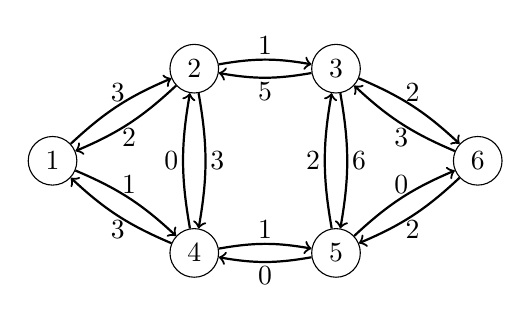
\begin{tikzpicture}[scale=0.9,label distance=-2mm]
\node[draw, circle] (1) at (1,1.3) {$1$};
\node[draw, circle] (2) at (3,2.6) {$2$};
\node[draw, circle] (3) at (5,2.6) {$3$};
\node[draw, circle] (4) at (7,1.3) {$6$};
\node[draw, circle] (5) at (3,0) {$4$};
\node[draw, circle] (6) at (5,0) {$5$};

\path[draw,thick,->] (1) edge [bend left=10] node[font=\small,label=3] {} (2);
\path[draw,thick,->] (2) edge [bend left=10] node[font=\small,label=below:2] {} (1);
\path[draw,thick,->] (2) edge [bend left=10] node[font=\small,label=1] {} (3);
\path[draw,thick,->] (3) edge [bend left=10] node[font=\small,label=below:5] {} (2);
\path[draw,thick,->] (3) edge [bend left=10] node[font=\small,label=2] {} (4);
\path[draw,thick,->] (4) edge [bend left=10] node[font=\small,label=below:3] {} (3);
\path[draw,thick,->] (1) edge [bend left=10] node[font=\small,label=1] {} (5);
\path[draw,thick,->] (5) edge [bend left=10] node[font=\small,label=below:3] {} (1);
\path[draw,thick,->] (5) edge [bend left=10] node[font=\small,label=1] {} (6);
\path[draw,thick,->] (6) edge [bend left=10] node[font=\small,label=below:0] {} (5);
\path[draw,thick,->] (6) edge [bend left=10] node[font=\small,label=0] {} (4);
\path[draw,thick,->] (4) edge [bend left=10] node[font=\small,label=below:2] {} (6);
\path[draw,thick,->] (5) edge [bend left=10] node[font=\small,label=left:0] {} (2);
\path[draw,thick,->] (2) edge [bend left=10] node[font=\small,label=right:3] {} (5);
\path[draw,thick,->] (3) edge [bend left=10] node[font=\small,label=right:6] {} (6);
\path[draw,thick,->] (6) edge [bend left=10] node[font=\small,label=left:2] {} (3);
\end{tikzpicture}
\end{center}
\end{samepage}

هنوز دو مرحله دیگر تا رسیدن به بیشینه شار نیاز است.
برای نمونه می‌توان مسیرهای
$1 \rightarrow 2 \rightarrow 3 \rightarrow 6$ و
$1 \rightarrow 4 \rightarrow 5 \rightarrow 3 \rightarrow 6$
را برگزید.
هر دو مسیر شار را به اندازه ۱ واحد افزایش می‌دهند
و گراف نهایی به صورت زیر خواهد بود:

\begin{center}
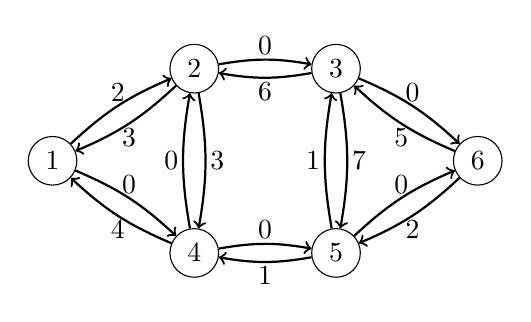
\begin{tikzpicture}[scale=0.9,label distance=-2mm]
\node[draw, circle] (1) at (1,1.3) {$1$};
\node[draw, circle] (2) at (3,2.6) {$2$};
\node[draw, circle] (3) at (5,2.6) {$3$};
\node[draw, circle] (4) at (7,1.3) {$6$};
\node[draw, circle] (5) at (3,0) {$4$};
\node[draw, circle] (6) at (5,0) {$5$};

\path[draw,thick,->] (1) edge [bend left=10] node[font=\small,label=2] {} (2);
\path[draw,thick,->] (2) edge [bend left=10] node[font=\small,label=below:3] {} (1);
\path[draw,thick,->] (2) edge [bend left=10] node[font=\small,label=0] {} (3);
\path[draw,thick,->] (3) edge [bend left=10] node[font=\small,label=below:6] {} (2);
\path[draw,thick,->] (3) edge [bend left=10] node[font=\small,label=0] {} (4);
\path[draw,thick,->] (4) edge [bend left=10] node[font=\small,label=below:5] {} (3);
\path[draw,thick,->] (1) edge [bend left=10] node[font=\small,label=0] {} (5);
\path[draw,thick,->] (5) edge [bend left=10] node[font=\small,label=below:4] {} (1);
\path[draw,thick,->] (5) edge [bend left=10] node[font=\small,label=0] {} (6);
\path[draw,thick,->] (6) edge [bend left=10] node[font=\small,label=below:1] {} (5);
\path[draw,thick,->] (6) edge [bend left=10] node[font=\small,label=0] {} (4);
\path[draw,thick,->] (4) edge [bend left=10] node[font=\small,label=below:2] {} (6);
\path[draw,thick,->] (5) edge [bend left=10] node[font=\small,label=left:0] {} (2);
\path[draw,thick,->] (2) edge [bend left=10] node[font=\small,label=right:3] {} (5);
\path[draw,thick,->] (3) edge [bend left=10] node[font=\small,label=right:7] {} (6);
\path[draw,thick,->] (6) edge [bend left=10] node[font=\small,label=left:1] {} (3);
\end{tikzpicture}
\end{center}

دیگر امکان افزایش شار وجود ندارد،
زیرا مسیری با وزن یال‌های مثبت از مبدأ
به مقصد موجود نیست.
بنابراین، الگوریتم پایان می‌یابد و بیشینه شار برابر ۷ است.

\subsubsection{یافتن مسیرها}

الگوریتم فورد--فالکرسون مشخص نمی‌کند که
مسیرهای افزایندهٔ شار چگونه باید انتخاب شوند.
در هر حال، الگوریتم دیر یا زود متوقف خواهد شد
و بیشینه شار را به‌درستی پیدا می‌کند.
با این وجود، کارایی الگوریتم به
نحوهٔ انتخاب مسیرها وابسته است.

یک روش ساده برای یافتن مسیرها استفاده از جستجوی اول‌سطح عمق است.
معمولاً این روش به‌خوبی کار می‌کند، اما در بدترین حالت،
هر مسیر شار را تنها به اندازهٔ ۱ واحد افزایش می‌دهد
و الگوریتم کند عمل خواهد کرد.
خوشبختانه می‌توان با استفاده از
یکی از فنون زیر از این وضعیت جلوگیری کرد:

\index{الگوریتم ادموندز--کارپ}

\key{الگوریتم ادموندز--کارپ} \cite{edm72}
هر مسیر را طوری انتخاب می‌کند که تعداد یال‌های
آن مسیر کمترین مقدار ممکن باشد.
این کار با به‌کارگیری جستجوی اول‌سطح به‌جای
جستجوی اول‌عمق برای یافتن مسیرها انجام‌پذیر است.
می‌توان اثبات کرد این امر متضمن افزایش
سریع شار است و پیچیدگی زمانی
الگوریتم برابر $O(m^2 n)$ خواهد بود.

\index{الگوریتم مقیاس‌بندی}

\key{الگوریتم مقیاس‌بندی} \cite{ahu91} از جستجوی اول‌عمق
جهت یافتن مسیرهایی استفاده می‌کند که در آن‌ها وزن هر یال
دست‌کم برابر با یک مقدار آستانه است.
در آغاز، مقدار آستانه عدد بزرگی در نظر گرفته می‌شود،
مثلاً مجموع تمام وزن‌های یال‌های گراف.
هر بار که یافتن مسیر ناممکن گردد،
مقدار آستانه بر ۲ تقسیم می‌شود.
پیچیدگی زمانی الگوریتم $O(m^2 \log c)$ است
که در آن $c$ نمایانگر مقدار آستانهٔ اولیه است.

در عمل، پیاده‌سازی الگوریتم مقیاس‌بندی آسان‌تر است،
زیرا می‌توان از جستجوی اول عمق برای یافتن مسیرها استفاده کرد.
هر دو الگوریتم برای مسائلی که معمولاً در مسابقات برنامه‌نویسی مطرح می‌شوند،
به اندازه کافی کارآمد هستند.

\subsubsection{برش‌های کمینه}

\index{برش کمینه}

مشخص می‌شود به محض اینکه الگوریتم فورد–فالکرسون
شار بیشینه را پیدا کند،
یک برش کمینه را نیز مشخص کرده است.
فرض کنید $A$ مجموعه‌ای از رأس‌ها باشد
که می‌توان با استفاده از یال‌های با وزن مثبت
از مبدأ به آن‌ها دسترسی پیدا کرد.
در گراف نمونه، $A$ شامل رأس‌های ۱، ۲ و ۴ است:

\begin{center}
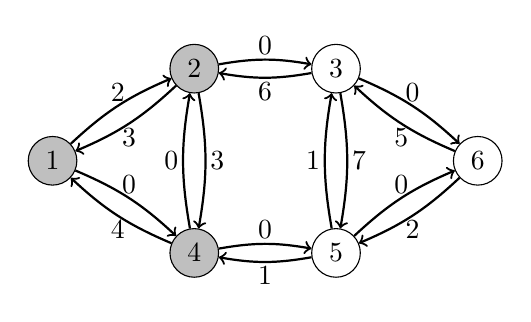
\begin{tikzpicture}[scale=0.9,label distance=-2mm]
\node[draw, circle,fill=lightgray] (1) at (1,1.3) {$1$};
\node[draw, circle,fill=lightgray] (2) at (3,2.6) {$2$};
\node[draw, circle] (3) at (5,2.6) {$3$};
\node[draw, circle] (4) at (7,1.3) {$6$};
\node[draw, circle,fill=lightgray] (5) at (3,0) {$4$};
\node[draw, circle] (6) at (5,0) {$5$};

\path[draw,thick,->] (1) edge [bend left=10] node[font=\small,label=2] {} (2);
\path[draw,thick,->] (2) edge [bend left=10] node[font=\small,label=below:3] {} (1);
\path[draw,thick,->] (2) edge [bend left=10] node[font=\small,label=0] {} (3);
\path[draw,thick,->] (3) edge [bend left=10] node[font=\small,label=below:6] {} (2);
\path[draw,thick,->] (3) edge [bend left=10] node[font=\small,label=0] {} (4);
\path[draw,thick,->] (4) edge [bend left=10] node[font=\small,label=below:5] {} (3);
\path[draw,thick,->] (1) edge [bend left=10] node[font=\small,label=0] {} (5);
\path[draw,thick,->] (5) edge [bend left=10] node[font=\small,label=below:4] {} (1);
\path[draw,thick,->] (5) edge [bend left=10] node[font=\small,label=0] {} (6);
\path[draw,thick,->] (6) edge [bend left=10] node[font=\small,label=below:1] {} (5);
\path[draw,thick,->] (6) edge [bend left=10] node[font=\small,label=0] {} (4);
\path[draw,thick,->] (4) edge [bend left=10] node[font=\small,label=below:2] {} (6);
\path[draw,thick,->] (5) edge [bend left=10] node[font=\small,label=left:0] {} (2);
\path[draw,thick,->] (2) edge [bend left=10] node[font=\small,label=right:3] {} (5);
\path[draw,thick,->] (3) edge [bend left=10] node[font=\small,label=right:7] {} (6);
\path[draw,thick,->] (6) edge [bend left=10] node[font=\small,label=left:1] {} (3);
\end{tikzpicture}
\end{center}

اکنون برش کمینه شامل یال‌هایی از گراف اصلی است
که از رأسی در $A$ شروع شده، به رأسی خارج از $A$ ختم می‌شوند،
و ظرفیت آن‌ها در شار بیشینه به طور کامل
استفاده شده است.
در گراف فوق، این یال‌ها
$2 \rightarrow 3$ و $4 \rightarrow 5$ هستند
که متناظر با برش کمینه $6+1=7$ می‌باشند.

چرا شار تولید شده توسط الگوریتم بیشینه است
و چرا برش کمینه است؟
دلیل آن این است که یک گراف نمی‌تواند
شامل شاری باشد که اندازه آن از وزن
هر برشی از گراف بزرگتر باشد.
بنابراین، همواره هنگامی که یک شار و یک برش هم‌اندازه باشند،
آن‌ها شار بیشینه و برش کمینه هستند.

برش دلخواهی از گراف را در نظر بگیرید
به طوری که مبدأ متعلق به $A$ باشد،
مقصد متعلق به $B$ باشد
و یال‌هایی بین این دو مجموعه وجود داشته باشد:

\begin{center}
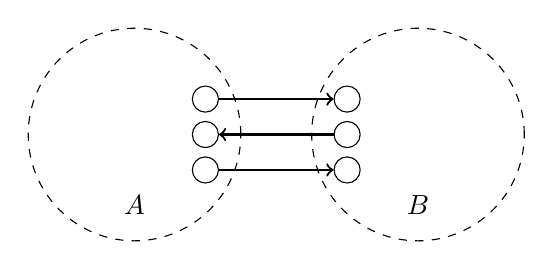
\begin{tikzpicture}[scale=0.9]
\draw[dashed] (-2,0) circle (1.5);
\draw[dashed] (2,0) circle (1.5);

\node at (-2,-1) {$A$};
\node at (2,-1) {$B$};

\node[draw, circle] (1) at (-1,0.5) {};
\node[draw, circle] (2) at (-1,0) {};
\node[draw, circle] (3) at (-1,-0.5) {};
\node[draw, circle] (4) at (1,0.5) {};
\node[draw, circle] (5) at (1,0) {};
\node[draw, circle] (6) at (1,-0.5) {};

\path[draw,thick,->] (1) -- (4);
\path[draw,thick,->] (5) -- (2);
\path[draw,thick,->] (3) -- (6);

\end{tikzpicture}
\end{center}

اندازه برش مجموع یال‌هایی است که
از $A$ به $B$ می‌روند.
این مقدار کران بالایی برای جریان
در گراف است، زیرا جریان باید
از $A$ به $B$ عبور کند.
بنابراین اندازه بیشینه شار کوچک‌تر یا مساوی
اندازه هر برشی در گراف است.

از طرف دیگر، الگوریتم فورد-فالکرسون
جریانی تولید می‌کند که اندازه‌اش \emph{دقیقاً} برابر
با اندازه یک برش در گراف است.
بنابراین، این جریان باید بیشینه شار
و آن برش باید کمینه برش باشد.

\section{مسیرهای مجزا}

بسیاری از مسائل گراف را می‌توان با کاهش
آن‌ها به مسئله بیشینه شار حل کرد.
اولین نمونه از چنین مسئله‌ای
به این صورت است: یک گراف جهت‌دار
با یک مبدأ و یک مقصد داده شده است،
و وظیفه ما یافتن بیشینه تعداد
مسیرهای مجزا از مبدأ به مقصد است.

\subsubsection{مسیرهای مجزا از یال}

ابتدا بر روی مسئله یافتن
بیشینه تعداد
\key{مسیرهای مجزا از یال} از مبدأ به مقصد تمرکز می‌کنیم.
این بدان معناست که باید مجموعه‌ای از مسیرها را تشکیل دهیم
به طوری که هر یال حداکثر در یک مسیر ظاهر شود.

به عنوان مثال، گراف زیر را در نظر بگیرید:
\begin{center}
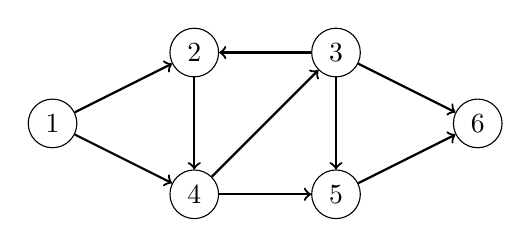
\begin{tikzpicture}[scale=0.9]
\node[draw, circle] (1) at (1,2) {$1$};
\node[draw, circle] (2) at (3,3) {$2$};
\node[draw, circle] (3) at (5,3) {$3$};
\node[draw, circle] (4) at (3,1) {$4$};
\node[draw, circle] (5) at (5,1) {$5$};
\node[draw, circle] (6) at (7,2) {$6$};
\path[draw,thick,->] (1) -- (2);
\path[draw,thick,->] (1) -- (4);
\path[draw,thick,->] (2) -- (4);
\path[draw,thick,->] (3) -- (2);
\path[draw,thick,->] (3) -- (5);
\path[draw,thick,->] (3) -- (6);
\path[draw,thick,->] (4) -- (3);
\path[draw,thick,->] (4) -- (5);
\path[draw,thick,->] (5) -- (6);
\end{tikzpicture}
\end{center}

در این گراف، بیشینه تعداد مسیرهای مجزا از یال
برابر ۲ است.
می‌توانیم مسیرهای
$1 \rightarrow 2 \rightarrow 4 \rightarrow 3 \rightarrow 6$
و $1 \rightarrow 4 \rightarrow 5 \rightarrow 6$ را به صورت زیر انتخاب کنیم:

\begin{center}
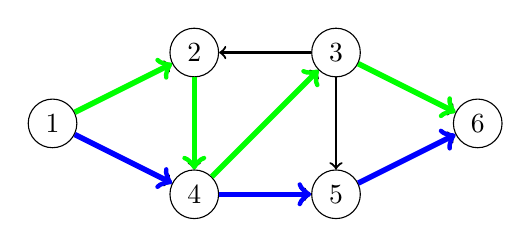
\begin{tikzpicture}[scale=0.9]
\node[draw, circle] (1) at (1,2) {$1$};
\node[draw, circle] (2) at (3,3) {$2$};
\node[draw, circle] (3) at (5,3) {$3$};
\node[draw, circle] (4) at (3,1) {$4$};
\node[draw, circle] (5) at (5,1) {$5$};
\node[draw, circle] (6) at (7,2) {$6$};
\path[draw,thick,->] (1) -- (2);
\path[draw,thick,->] (1) -- (4);
\path[draw,thick,->] (2) -- (4);
\path[draw,thick,->] (3) -- (2);
\path[draw,thick,->] (3) -- (5);
\path[draw,thick,->] (3) -- (6);
\path[draw,thick,->] (4) -- (3);
\path[draw,thick,->] (4) -- (5);
\path[draw,thick,->] (5) -- (6);

\path[draw=green,thick,->,line width=2pt] (1) -- (2);
\path[draw=green,thick,->,line width=2pt] (2) -- (4);
\path[draw=green,thick,->,line width=2pt] (4) -- (3);
\path[draw=green,thick,->,line width=2pt] (3) -- (6);

\path[draw=blue,thick,->,line width=2pt] (1) -- (4);
\path[draw=blue,thick,->,line width=2pt] (4) -- (5);
\path[draw=blue,thick,->,line width=2pt] (5) -- (6);
\end{tikzpicture}
\end{center}

مشخص می‌شود که حداکثر تعداد
مسیرهای یال‌مجزا
برابر با بیشینه شار گراف است،
با این فرض که ظرفیت هر یال برابر یک باشد.
پس از ساخت بیشینه شار،
مسیرهای یال‌مجزا را می‌توان به صورت حریصانه
با دنبال کردن مسیرها از مبدأ تا مقصد یافت.

\subsubsection{مسیرهای رأس‌مجزا}

حال مسئله دیگری را بررسی می‌کنیم:
یافتن بیشینه تعداد
\key{مسیرهای رأس‌مجزا} از مبدأ
به مقصد.
در این مسئله، هر رأس،
به جز مبدأ و مقصد،
می‌تواند حداکثر در یک مسیر ظاهر شود.
تعداد مسیرهای رأس‌مجزا
ممکن است کمتر از تعداد
مسیرهای یال‌مجزا باشد.

برای نمونه، در گراف قبلی،
بیشینه تعداد مسیرهای رأس‌مجزا برابر ۱ است:

\begin{center}
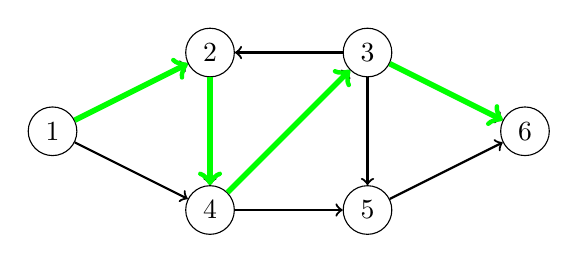
\begin{tikzpicture}
\node[draw, circle] (1) at (1,2) {$1$};
\node[draw, circle] (2) at (3,3) {$2$};
\node[draw, circle] (3) at (5,3) {$3$};
\node[draw, circle] (4) at (3,1) {$4$};
\node[draw, circle] (5) at (5,1) {$5$};
\node[draw, circle] (6) at (7,2) {$6$};
\path[draw,thick,->] (1) -- (2);
\path[draw,thick,->] (1) -- (4);
\path[draw,thick,->] (2) -- (4);
\path[draw,thick,->] (3) -- (2);
\path[draw,thick,->] (3) -- (5);
\path[draw,thick,->] (3) -- (6);
\path[draw,thick,->] (4) -- (3);
\path[draw,thick,->] (4) -- (5);
\path[draw,thick,->] (5) -- (6);

\path[draw=green,thick,->,line width=2pt] (1) -- (2);
\path[draw=green,thick,->,line width=2pt] (2) -- (4);
\path[draw=green,thick,->,line width=2pt] (4) -- (3);
\path[draw=green,thick,->,line width=2pt] (3) -- (6);
\end{tikzpicture}
\end{center}

این مسئله را نیز می‌توان به مسئله بیشینه شار کاهش داد.
از آنجا که هر رأس می‌تواند حداکثر در یک مسیر ظاهر شود،
باید شاری را که از رأس‌ها عبور می‌کند محدود کنیم.
یک روش استاندارد برای این کار، تقسیم هر رأس به
دو رأس است به طوری که رأس نخست یال‌های ورودی
رأس اصلی را داشته باشد، رأس دوم یال‌های خروجی
رأس اصلی را شامل شود، و
یک یال جدید از رأس نخست
به رأس دوم وجود داشته باشد.

در مثال ما، گراف به صورت زیر تبدیل می‌شود:
\begin{center}
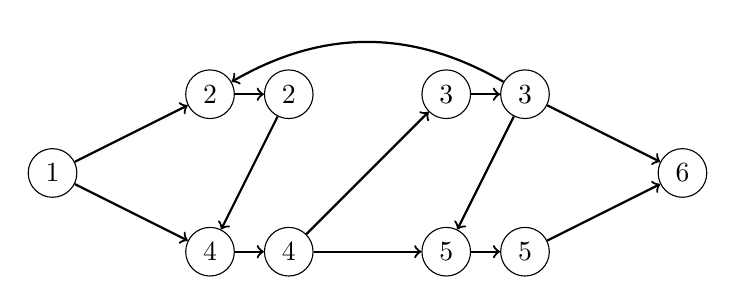
\begin{tikzpicture}
\node[draw, circle] (1) at (1,2) {$1$};

\node[draw, circle] (2a) at (3,3) {$2$};
\node[draw, circle] (3a) at (6,3) {$3$};
\node[draw, circle] (4a) at (3,1) {$4$};
\node[draw, circle] (5a) at (6,1) {$5$};

\node[draw, circle] (2b) at (4,3) {$2$};
\node[draw, circle] (3b) at (7,3) {$3$};
\node[draw, circle] (4b) at (4,1) {$4$};
\node[draw, circle] (5b) at (7,1) {$5$};

\node[draw, circle] (6) at (9,2) {$6$};

\path[draw,thick,->] (2a) -- (2b);
\path[draw,thick,->] (3a) -- (3b);
\path[draw,thick,->] (4a) -- (4b);
\path[draw,thick,->] (5a) -- (5b);

\path[draw,thick,->] (1) -- (2a);
\path[draw,thick,->] (1) -- (4a);
\path[draw,thick,->] (2b) -- (4a);
\path[draw,thick,->] (3b) edge [bend right=30] (2a);
\path[draw,thick,->] (3b) -- (5a);
\path[draw,thick,->] (3b) -- (6);
\path[draw,thick,->] (4b) -- (3a);
\path[draw,thick,->] (4b) -- (5a);
\path[draw,thick,->] (5b) -- (6);
\end{tikzpicture}
\end{center}

شار بیشینه برای گراف به صورت زیر است:
\begin{center}
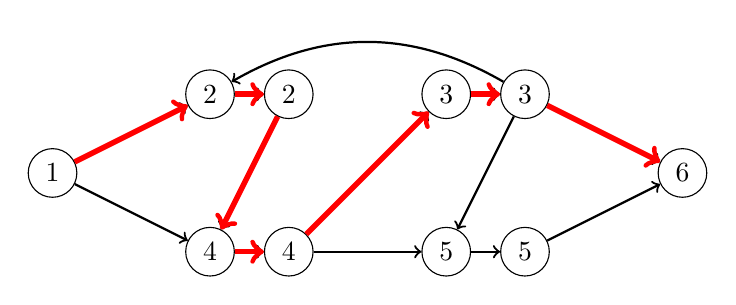
\begin{tikzpicture}
\node[draw, circle] (1) at (1,2) {$1$};

\node[draw, circle] (2a) at (3,3) {$2$};
\node[draw, circle] (3a) at (6,3) {$3$};
\node[draw, circle] (4a) at (3,1) {$4$};
\node[draw, circle] (5a) at (6,1) {$5$};

\node[draw, circle] (2b) at (4,3) {$2$};
\node[draw, circle] (3b) at (7,3) {$3$};
\node[draw, circle] (4b) at (4,1) {$4$};
\node[draw, circle] (5b) at (7,1) {$5$};

\node[draw, circle] (6) at (9,2) {$6$};

\path[draw,thick,->] (2a) -- (2b);
\path[draw,thick,->] (3a) -- (3b);
\path[draw,thick,->] (4a) -- (4b);
\path[draw,thick,->] (5a) -- (5b);

\path[draw,thick,->] (1) -- (2a);
\path[draw,thick,->] (1) -- (4a);
\path[draw,thick,->] (2b) -- (4a);
\path[draw,thick,->] (3b) edge [bend right=30] (2a);
\path[draw,thick,->] (3b) -- (5a);
\path[draw,thick,->] (3b) -- (6);
\path[draw,thick,->] (4b) -- (3a);
\path[draw,thick,->] (4b) -- (5a);
\path[draw,thick,->] (5b) -- (6);

\path[draw=red,thick,->,line width=2pt] (1) -- (2a);
\path[draw=red,thick,->,line width=2pt] (2a) -- (2b);
\path[draw=red,thick,->,line width=2pt] (2b) -- (4a);
\path[draw=red,thick,->,line width=2pt] (4a) -- (4b);
\path[draw=red,thick,->,line width=2pt] (4b) -- (3a);
\path[draw=red,thick,->,line width=2pt] (3a) -- (3b);
\path[draw=red,thick,->,line width=2pt] (3b) -- (6);
\end{tikzpicture}
\end{center}

بنابراین بیشینه تعداد مسیرهای مجزا از راس
از مبدا به مقصد برابر با ۱ است.

\section{تطابق‌های بیشینه}

\index{matching@تطابق}
\index{maximum matching@تطابق بیشینه}

مسئله \key{تطابق بیشینه} به دنبال یافتن
مجموعه‌ای با بیشترین اندازه از جفت‌راس‌ها در گراف بدون جهت است
به طوری که هر جفت با یک یال متصل باشد و
هر راس حداکثر به یک جفت تعلق داشته باشد.

الگوریتم‌های چندجمله‌ای برای یافتن تطابق بیشینه در گراف‌های کلی وجود دارند \cite{edm65}، اما این الگوریتم‌ها پیچیده‌اند و به‌ندرت در مسابقات برنامه‌نویسی دیده می‌شوند.
با این حال، در گراف‌های دوبخشی، مسئله تطابق بیشینه بسیار ساده‌تر حل می‌شود، زیرا می‌توانیم آن را به مسئله شار بیشینه تبدیل کنیم.

\subsubsection{یافتن تطابق‌های بیشینه}

گره‌های یک گراف دوبخشی همواره می‌توانند به دو گروه تقسیم شوند، به طوری که تمام یال‌های گراف از گروه سمت چپ به گروه سمت راست بروند.
به عنوان مثال، در گراف دوبخشی زیر، گروه‌ها $\{1,2,3,4\}$ و $\{5,6,7,8\}$ هستند.

\begin{center}
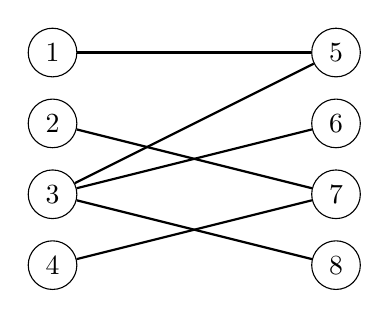
\begin{tikzpicture}[scale=0.60]
\node[draw, circle] (1) at (2,4.5) {1};
\node[draw, circle] (2) at (2,3) {2};
\node[draw, circle] (3) at (2,1.5) {3};
\node[draw, circle] (4) at (2,0) {4};
\node[draw, circle] (5) at (8,4.5) {5};
\node[draw, circle] (6) at (8,3) {6};
\node[draw, circle] (7) at (8,1.5) {7};
\node[draw, circle] (8) at (8,0) {8};

\path[draw,thick,-] (1) -- (5);
\path[draw,thick,-] (2) -- (7);
\path[draw,thick,-] (3) -- (5);
\path[draw,thick,-] (3) -- (6);
\path[draw,thick,-] (3) -- (8);
\path[draw,thick,-] (4) -- (7);
\end{tikzpicture}
\end{center}
اندازه تطابق بیشینه این گراف برابر ۳ است:
\begin{center}
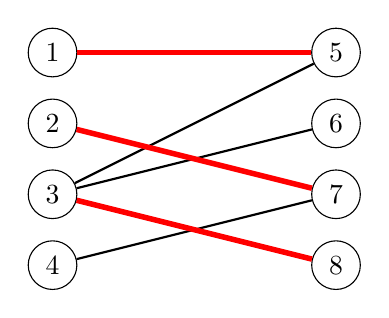
\begin{tikzpicture}[scale=0.60]
\node[draw, circle] (1) at (2,4.5) {1};
\node[draw, circle] (2) at (2,3) {2};
\node[draw, circle] (3) at (2,1.5) {3};
\node[draw, circle] (4) at (2,0) {4};
\node[draw, circle] (5) at (8,4.5) {5};
\node[draw, circle] (6) at (8,3) {6};
\node[draw, circle] (7) at (8,1.5) {7};
\node[draw, circle] (8) at (8,0) {8};

\path[draw,thick,-] (1) -- (5);
\path[draw,thick,-] (2) -- (7);
\path[draw,thick,-] (3) -- (5);
\path[draw,thick,-] (3) -- (6);
\path[draw,thick,-] (3) -- (8);
\path[draw,thick,-] (4) -- (7);

\path[draw=red,thick,-,line width=2pt] (1) -- (5);
\path[draw=red,thick,-,line width=2pt] (2) -- (7);
\path[draw=red,thick,-,line width=2pt] (3) -- (8);
\end{tikzpicture}
\end{center}

می‌توانیم مسئله تطابق بیشینه دوبخشی را با افزودن دو گره جدید به گراف به مسئله شار بیشینه تقلیل دهیم: یک مبدأ و یک مقصد.
همچنین یال‌هایی از مبدأ به هر گره سمت چپ، و از هر گره سمت راست به مقصد اضافه می‌کنیم.
پس از این کار، اندازه شار بیشینه در گراف برابر با اندازه تطابق بیشینه در گراف اولیه خواهد بود.

برای نمونه، تقلیل گراف بالا به شکل زیر است:
\begin{center}
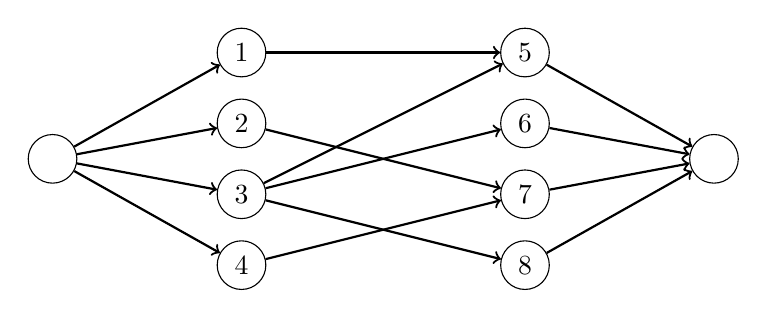
\begin{tikzpicture}[scale=0.60]
\node[draw, circle] (1) at (2,4.5) {1};
\node[draw, circle] (2) at (2,3) {2};
\node[draw, circle] (3) at (2,1.5) {3};
\node[draw, circle] (4) at (2,0) {4};
\node[draw, circle] (5) at (8,4.5) {5};
\node[draw, circle] (6) at (8,3) {6};
\node[draw, circle] (7) at (8,1.5) {7};
\node[draw, circle] (8) at (8,0) {8};

\node[draw, circle] (a) at (-2,2.25) {\phantom{0}};
\node[draw, circle] (b) at (12,2.25) {\phantom{0}};

\path[draw,thick,->] (1) -- (5);
\path[draw,thick,->] (2) -- (7);
\path[draw,thick,->] (3) -- (5);
\path[draw,thick,->] (3) -- (6);
\path[draw,thick,->] (3) -- (8);
\path[draw,thick,->] (4) -- (7);

\path[draw,thick,->] (a) -- (1);
\path[draw,thick,->] (a) -- (2);
\path[draw,thick,->] (a) -- (3);
\path[draw,thick,->] (a) -- (4);
\path[draw,thick,->] (5) -- (b);
\path[draw,thick,->] (6) -- (b);
\path[draw,thick,->] (7) -- (b);
\path[draw,thick,->] (8) -- (b);
\end{tikzpicture}
\end{center}

شار بیشینه این گراف به صورت زیر است:
\begin{center}
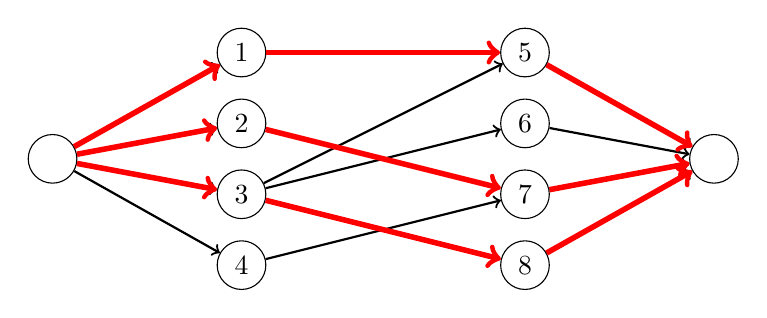
\begin{tikzpicture}[scale=0.60]
\node[draw, circle] (1) at (2,4.5) {1};
\node[draw, circle] (2) at (2,3) {2};
\node[draw, circle] (3) at (2,1.5) {3};
\node[draw, circle] (4) at (2,0) {4};
\node[draw, circle] (5) at (8,4.5) {5};
\node[draw, circle] (6) at (8,3) {6};
\node[draw, circle] (7) at (8,1.5) {7};
\node[draw, circle] (8) at (8,0) {8};

\node[draw, circle] (a) at (-2,2.25) {\phantom{0}};
\node[draw, circle] (b) at (12,2.25) {\phantom{0}};

\path[draw,thick,->] (3) -- (5);
\path[draw,thick,->] (3) -- (6);
\path[draw,thick,->] (4) -- (7);

\path[draw,thick,->] (a) -- (1);
\path[draw,thick,->] (a) -- (2);
\path[draw,thick,->] (a) -- (3);
\path[draw,thick,->] (a) -- (4);
\path[draw,thick,->] (5) -- (b);
\path[draw,thick,->] (6) -- (b);
\path[draw,thick,->] (7) -- (b);
\path[draw,thick,->] (8) -- (b);

\path[draw=red,thick,->,line width=2pt] (1) -- (5);
\path[draw=red,thick,->,line width=2pt] (2) -- (7);
\path[draw=red,thick,->,line width=2pt] (3) -- (8);

\path[draw=red,thick,->,line width=2pt] (a) -- (1);
\path[draw=red,thick,->,line width=2pt] (a) -- (2);
\path[draw=red,thick,->,line width=2pt] (a) -- (3);

\path[draw=red,thick,->,line width=2pt] (5) -- (b);
\path[draw=red,thick,->,line width=2pt] (7) -- (b);
\path[draw=red,thick,->,line width=2pt] (8) -- (b);

\end{tikzpicture}
\end{center}

\subsubsection{قضیه هال}

\index{Hall's theorem@قضیه هال}
\index{perfect matching@تطابق کامل}

از \key{قضیه هال} می‌توان برای تشخیص وجود تطابقی در یک گراف دوبخشی استفاده کرد که تمام رأس‌های سمت چپ یا راست را شامل شود.
اگر تعداد رأس‌های چپ و راست برابر باشد، قضیه هال مشخص می‌کند آیا امکان ساخت یک \key{تطابق کامل} شامل تمام رأس‌های گراف وجود دارد یا خیر.

فرض کنید می‌خواهیم تطابقی شامل تمام رأس‌های سمت چپ بیابیم.
فرض کنید $X$ زیرمجموعه‌ای دلخواه از رأس‌های سمت چپ و $f(X)$ مجموعه همسایه‌های آن‌ها باشد.
طبق قضیه هال، تطابقی شامل تمام رأس‌های سمت چپ وجود دارد اگر و تنها اگر به ازای هر $X$، شرط $|X| \le |f(X)|$ برقرار باشد.

قضیه هال را در گراف مثال بررسی می‌کنیم.
ابتدا فرض کنید $X=\{1,3\}$ باشد که نتیجه می‌دهد $f(X)=\{5,6,8\}$:

\begin{center}
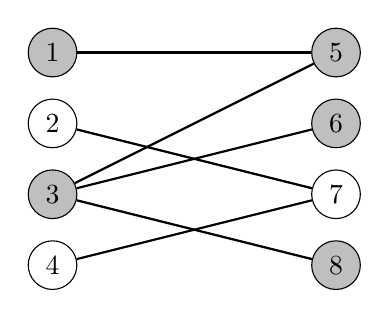
\begin{tikzpicture}[scale=0.60]
\node[draw, circle, fill=lightgray] (1) at (2,4.5) {1};
\node[draw, circle] (2) at (2,3) {2};
\node[draw, circle, fill=lightgray] (3) at (2,1.5) {3};
\node[draw, circle] (4) at (2,0) {4};
\node[draw, circle, fill=lightgray] (5) at (8,4.5) {5};
\node[draw, circle, fill=lightgray] (6) at (8,3) {6};
\node[draw, circle] (7) at (8,1.5) {7};
\node[draw, circle, fill=lightgray] (8) at (8,0) {8};

\path[draw,thick,-] (1) -- (5);
\path[draw,thick,-] (2) -- (7);
\path[draw,thick,-] (3) -- (5);
\path[draw,thick,-] (3) -- (6);
\path[draw,thick,-] (3) -- (8);
\path[draw,thick,-] (4) -- (7);
\end{tikzpicture}
\end{center}

شرط قضیه هال برقرار است، زیرا
$|X|=2$ و $|f(X)|=3$.
سپس فرض کنید $X=\{2,4\}$ باشد که نتیجه می‌دهد $f(X)=\{7\}$:

\begin{center}
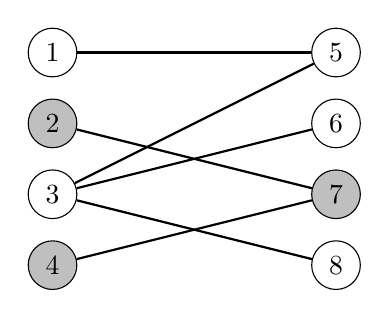
\begin{tikzpicture}[scale=0.60]
\node[draw, circle] (1) at (2,4.5) {1};
\node[draw, circle, fill=lightgray] (2) at (2,3) {2};
\node[draw, circle] (3) at (2,1.5) {3};
\node[draw, circle, fill=lightgray] (4) at (2,0) {4};
\node[draw, circle] (5) at (8,4.5) {5};
\node[draw, circle] (6) at (8,3) {6};
\node[draw, circle, fill=lightgray] (7) at (8,1.5) {7};
\node[draw, circle] (8) at (8,0) {8};

\path[draw,thick,-] (1) -- (5);
\path[draw,thick,-] (2) -- (7);
\path[draw,thick,-] (3) -- (5);
\path[draw,thick,-] (3) -- (6);
\path[draw,thick,-] (3) -- (8);
\path[draw,thick,-] (4) -- (7);
\end{tikzpicture}
\end{center}

در این حالت، $|X|=2$ و $|f(X)|=1$ است،
بنابراین شرط قضیه هال برقرار نیست.
یعنی تشکیل تطابق کامل برای این گراف ممکن نیست.
این نتیجه دور از انتظار نیست، چون از قبل
می‌دانیم تطابق بیشینه گراف ۳ است نه ۴.

اگر شرط قضیه هال برقرار نباشد،
مجموعه $X$ نشان می‌دهد \emph{چرا}
نمی‌توان چنین تطابقی تشکیل داد.
چون $X$ گره‌های بیشتری نسبت به $f(X)$ دارد،
جفت کافی برای همه گره‌های $X$ وجود ندارد.
مثلاً در گراف بالا، هر دو گره ۲ و ۴
باید به گره ۷ متصل شوند که شدنی نیست.

\subsubsection{قضیه کونیگ}

\index{قضیه کونیگ}
\index{پوشش راس}
\index{حداقل پوشش راس}

یک \key{پوشش راس کمینه} برای گراف،
مجموعه‌ای کمینه از گره‌هاست که هر یال گراف
حداقل یک سرش در آن مجموعه باشد.
در گراف کلی، پیدا کردن پوشش راس کمینه
یک مسئله NP-hard است.
اما اگر گراف دوبخشی باشد،
\key{قضیه کونیگ} می‌گوید اندازه پوشش راس کمینه
و اندازه تطابق بیشینه همیشه برابرند.
بنابراین می‌توان اندازه پوشش راس کمینه را
با الگوریتم شار بیشینه محاسبه کرد.

گراف زیر با تطابق بیشینه به اندازه ۳ را در نظر بگیرید:
\begin{center}
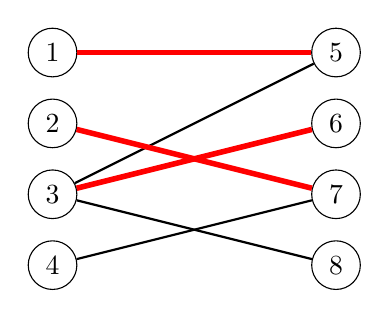
\begin{tikzpicture}[scale=0.60]
\node[draw, circle] (1) at (2,4.5) {1};
\node[draw, circle] (2) at (2,3) {2};
\node[draw, circle] (3) at (2,1.5) {3};
\node[draw, circle] (4) at (2,0) {4};
\node[draw, circle] (5) at (8,4.5) {5};
\node[draw, circle] (6) at (8,3) {6};
\node[draw, circle] (7) at (8,1.5) {7};
\node[draw, circle] (8) at (8,0) {8};

\path[draw,thick,-] (1) -- (5);
\path[draw,thick,-] (2) -- (7);
\path[draw,thick,-] (3) -- (5);
\path[draw,thick,-] (3) -- (6);
\path[draw,thick,-] (3) -- (8);
\path[draw,thick,-] (4) -- (7);

\path[draw=red,thick,-,line width=2pt] (1) -- (5);
\path[draw=red,thick,-,line width=2pt] (2) -- (7);
\path[draw=red,thick,-,line width=2pt] (3) -- (6);
\end{tikzpicture}
\end{center}
قضیه کونیگ بیان می‌کند اندازه پوشش راسی کمینه نیز برابر ۳ است.
چنین پوششی را می‌توان به صورت زیر ساخت:

\begin{center}
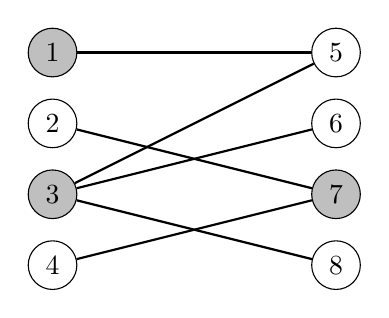
\begin{tikzpicture}[scale=0.60]
\node[draw, circle, fill=lightgray] (1) at (2,4.5) {1};
\node[draw, circle] (2) at (2,3) {2};
\node[draw, circle, fill=lightgray] (3) at (2,1.5) {3};
\node[draw, circle] (4) at (2,0) {4};
\node[draw, circle] (5) at (8,4.5) {5};
\node[draw, circle] (6) at (8,3) {6};
\node[draw, circle, fill=lightgray] (7) at (8,1.5) {7};
\node[draw, circle] (8) at (8,0) {8};

\path[draw,thick,-] (1) -- (5);
\path[draw,thick,-] (2) -- (7);
\path[draw,thick,-] (3) -- (5);
\path[draw,thick,-] (3) -- (6);
\path[draw,thick,-] (3) -- (8);
\path[draw,thick,-] (4) -- (7);
\end{tikzpicture}
\end{center}

\index{مجموعه مستقل}
\index{مجموعه مستقل بیشینه}

راس‌هایی که به پوشش راسی کمینه تعلق \emph{ندارند}،
تشکیل یک \key{مجموعه مستقل بیشینه} می‌دهند.
این بزرگ‌ترین مجموعه ممکن از راس‌ها است
به‌طوری‌که هیچ دو راسی در مجموعه
با یک یال به هم متصل نباشند.
یافتن مجموعه مستقل بیشینه در گراف عمومی مسئله‌ای NP-hard است،
اما در گراف دوبخشی می‌توان از قضیه کونیگ برای حل کارآمد مسئله استفاده کرد.
در گراف نمونه، مجموعه مستقل بیشینه به صورت زیر است:

\begin{center}
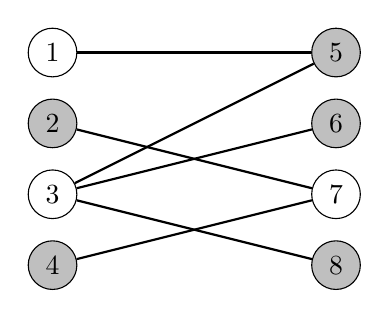
\begin{tikzpicture}[scale=0.60]
\node[draw, circle] (1) at (2,4.5) {1};
\node[draw, circle, fill=lightgray] (2) at (2,3) {2};
\node[draw, circle] (3) at (2,1.5) {3};
\node[draw, circle, fill=lightgray] (4) at (2,0) {4};
\node[draw, circle, fill=lightgray] (5) at (8,4.5) {5};
\node[draw, circle, fill=lightgray] (6) at (8,3) {6};
\node[draw, circle] (7) at (8,1.5) {7};
\node[draw, circle, fill=lightgray] (8) at (8,0) {8};

\path[draw,thick,-] (1) -- (5);
\path[draw,thick,-] (2) -- (7);
\path[draw,thick,-] (3) -- (5);
\path[draw,thick,-] (3) -- (6);
\path[draw,thick,-] (3) -- (8);
\path[draw,thick,-] (4) -- (7);
\end{tikzpicture}
\end{center}

\section{پوشش‌های مسیری}

\index{پوشش مسیری}

یک \key{پوشش مسیری} (path cover) مجموعه‌ای از مسیرها در یک گراف است
به‌طوری که هر رأس گراف متعلق به حداقل یک مسیر باشد.
مشخص می‌شود که در گراف‌های جهت‌دار بدون دور (DAG)،
می‌توان مسئله‌ی یافتن کمینه‌پوشش
مسیری را به مسئله‌ی یافتن بیشینه‌شار
در گرافی دیگر کاهش داد.

\subsubsection{پوشش مسیری رأس‌جدا}

در یک \key{پوشش مسیری رأس‌جدا} (node-disjoint path cover)،
هر رأس دقیقاً متعلق به یک مسیر است.
به عنوان مثال، گراف زیر را در نظر بگیرید:
\begin{center}
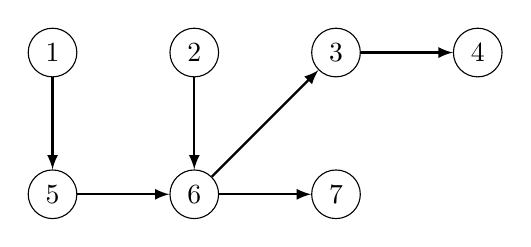
\begin{tikzpicture}[scale=0.9]
\node[draw, circle] (1) at (0,0) {1};
\node[draw, circle] (2) at (2,0) {2};
\node[draw, circle] (3) at (4,0) {3};
\node[draw, circle] (4) at (6,0) {4};
\node[draw, circle] (5) at (0,-2) {5};
\node[draw, circle] (6) at (2,-2) {6};
\node[draw, circle] (7) at (4,-2) {7};

\path[draw,thick,->,>=latex] (1) -- (5);
\path[draw,thick,->,>=latex] (2) -- (6);
\path[draw,thick,->,>=latex] (3) -- (4);
\path[draw,thick,->,>=latex] (5) -- (6);
\path[draw,thick,->,>=latex] (6) -- (3);
\path[draw,thick,->,>=latex] (6) -- (7);
\end{tikzpicture}
\end{center}

یک پوشش مسیری رأس‌جدای کمینه
برای این گراف
شامل سه مسیر است.
به عنوان مثال، می‌توانیم مسیرهای زیر را انتخاب کنیم:

\begin{center}
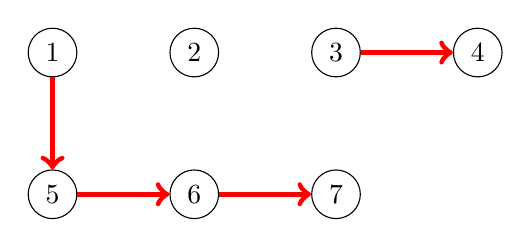
\begin{tikzpicture}[scale=0.9]
\node[draw, circle] (1) at (0,0) {1};
\node[draw, circle] (2) at (2,0) {2};
\node[draw, circle] (3) at (4,0) {3};
\node[draw, circle] (4) at (6,0) {4};
\node[draw, circle] (5) at (0,-2) {5};
\node[draw, circle] (6) at (2,-2) {6};
\node[draw, circle] (7) at (4,-2) {7};

\path[draw=red,thick,->,line width=2pt] (1) -- (5);
\path[draw=red,thick,->,line width=2pt] (5) -- (6);
\path[draw=red,thick,->,line width=2pt] (6) -- (7);
\path[draw=red,thick,->,line width=2pt] (3) -- (4);
\end{tikzpicture}
\end{center}

توجه کنید یکی از مسیرها فقط شامل رأس ۲ است،
بنابراین ممکن است یک مسیر اصلاً هیچ یالی نداشته باشد.

می‌توانیم با ساخت یک \emph{گراف تطابق}، پوشش مسیری رأس‌جدای کمینه را
بیابیم که در آن هر رأس
گراف اصلی با
دو رأس نمایش داده می‌شود: یک رأس چپ و یک رأس راست.
یالی از رأس چپ به رأس راست وجود دارد
اگر چنین یالی در گراف اصلی موجود باشد.
علاوه بر این، گراف تطابق شامل یک مبدأ و یک مقصد است،
و یال‌هایی از مبدأ به همه‌ی
رؤسای چپ و از همه‌ی رؤسای راست به مقصد وجود دارد.

یک بیشینه‌تطابق در گراف حاصل متناظر
با یک کمینه‌پوشش مسیری رأس‌جدا در
گراف اصلی است.
به عنوان مثال، گراف تطابق زیر
برای گراف بالا شامل
یک بیشینه‌تطابق با اندازه‌ی ۴ است:

\begin{center}
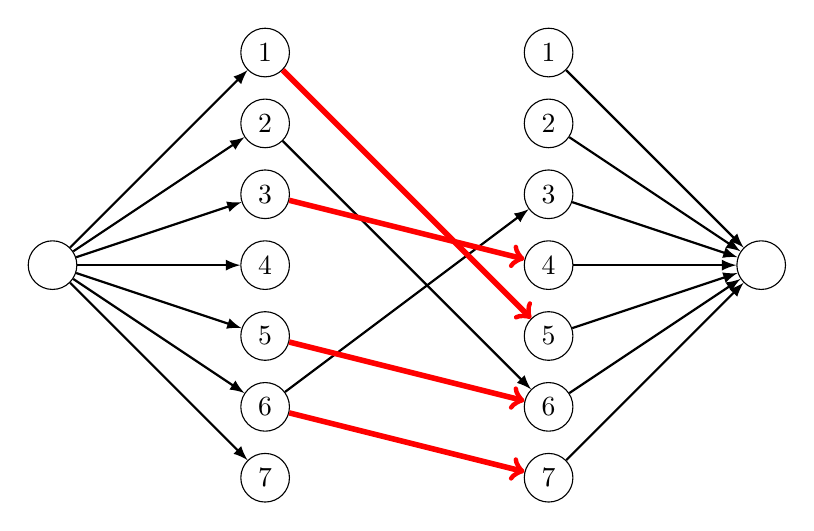
\begin{tikzpicture}[scale=0.9]
\node[draw, circle] (1a) at (0,6) {1};
\node[draw, circle] (2a) at (0,5) {2};
\node[draw, circle] (3a) at (0,4) {3};
\node[draw, circle] (4a) at (0,3) {4};
\node[draw, circle] (5a) at (0,2) {5};
\node[draw, circle] (6a) at (0,1) {6};
\node[draw, circle] (7a) at (0,0) {7};

\node[draw, circle] (1b) at (4,6) {1};
\node[draw, circle] (2b) at (4,5) {2};
\node[draw, circle] (3b) at (4,4) {3};
\node[draw, circle] (4b) at (4,3) {4};
\node[draw, circle] (5b) at (4,2) {5};
\node[draw, circle] (6b) at (4,1) {6};
\node[draw, circle] (7b) at (4,0) {7};

\node[draw, circle] (a) at (-3,3) {\phantom{0}};
\node[draw, circle] (b) at (7,3) {\phantom{0}};

%\path[draw,thick,->,>=latex] (1a) -- (5b);
\path[draw,thick,->,>=latex] (2a) -- (6b);
%\path[draw,thick,->,>=latex] (3a) -- (4b);
%\path[draw,thick,->,>=latex] (5a) -- (6b);
\path[draw,thick,->,>=latex] (6a) -- (3b);
%\path[draw,thick,->,>=latex] (6a) -- (7b);

\path[draw,thick,->,>=latex] (a) -- (1a);
\path[draw,thick,->,>=latex] (a) -- (2a);
\path[draw,thick,->,>=latex] (a) -- (3a);
\path[draw,thick,->,>=latex] (a) -- (4a);
\path[draw,thick,->,>=latex] (a) -- (5a);
\path[draw,thick,->,>=latex] (a) -- (6a);
\path[draw,thick,->,>=latex] (a) -- (7a);

\path[draw,thick,->,>=latex] (1b) -- (b);
\path[draw,thick,->,>=latex] (2b) -- (b);
\path[draw,thick,->,>=latex] (3b) -- (b);
\path[draw,thick,->,>=latex] (4b) -- (b);
\path[draw,thick,->,>=latex] (5b) -- (b);
\path[draw,thick,->,>=latex] (6b) -- (b);
\path[draw,thick,->,>=latex] (7b) -- (b);

\path[draw=red,thick,->,line width=2pt] (1a) -- (5b);
\path[draw=red,thick,->,line width=2pt] (5a) -- (6b);
\path[draw=red,thick,->,line width=2pt] (6a) -- (7b);
\path[draw=red,thick,->,line width=2pt] (3a) -- (4b);

\end{tikzpicture}
\end{center}

هر یال در تطابق بیشینه گراف تطابق، متناظر با یک یال در پوشش مسیری گره‌مجزای کمینه گراف اصلی است.
بنابراین، اندازه پوشش مسیری گره‌مجزای کمینه برابر با $n-c$ است،
که در آن $n$ تعداد گره‌های گراف اصلی
و $c$ اندازه تطابق بیشینه است.

\subsubsection{پوشش مسیری عمومی}

یک \key{پوشش مسیری عمومی} پوششی از مسیرها است
که در آن یک گره می‌تواند به بیش از یک مسیر تعلق داشته باشد.
یک پوشش مسیری عمومی کمینه ممکن است از یک پوشش مسیری گره‌مجزای کمینه کوچک‌تر باشد،
زیرا یک گره می‌تواند چندین بار در مسیرها استفاده شود.
دوباره گراف زیر را در نظر بگیرید:
\begin{center}
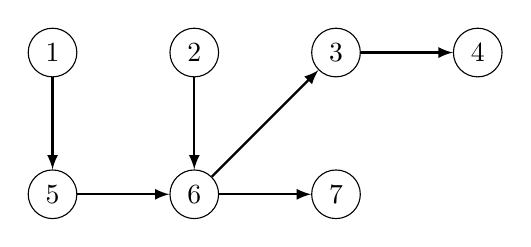
\begin{tikzpicture}[scale=0.9]
\node[draw, circle] (1) at (0,0) {1};
\node[draw, circle] (2) at (2,0) {2};
\node[draw, circle] (3) at (4,0) {3};
\node[draw, circle] (4) at (6,0) {4};
\node[draw, circle] (5) at (0,-2) {5};
\node[draw, circle] (6) at (2,-2) {6};
\node[draw, circle] (7) at (4,-2) {7};

\path[draw,thick,->,>=latex] (1) -- (5);
\path[draw,thick,->,>=latex] (2) -- (6);
\path[draw,thick,->,>=latex] (3) -- (4);
\path[draw,thick,->,>=latex] (5) -- (6);
\path[draw,thick,->,>=latex] (6) -- (3);
\path[draw,thick,->,>=latex] (6) -- (7);
\end{tikzpicture}
\end{center}

پوشش مسیر عمومی کمینه این گراف
شامل دو مسیر است.
برای نمونه، مسیر نخست می‌تواند به این صورت باشد:
\begin{center}
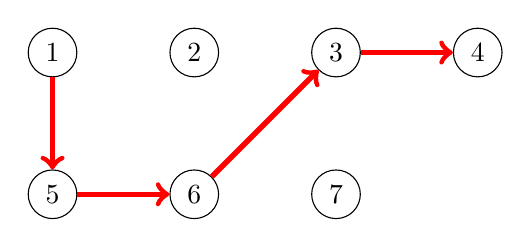
\begin{tikzpicture}[scale=0.9]
\node[draw, circle] (1) at (0,0) {1};
\node[draw, circle] (2) at (2,0) {2};
\node[draw, circle] (3) at (4,0) {3};
\node[draw, circle] (4) at (6,0) {4};
\node[draw, circle] (5) at (0,-2) {5};
\node[draw, circle] (6) at (2,-2) {6};
\node[draw, circle] (7) at (4,-2) {7};

\path[draw=red,thick,->,line width=2pt] (1) -- (5);
\path[draw=red,thick,->,line width=2pt] (5) -- (6);
\path[draw=red,thick,->,line width=2pt] (6) -- (3);
\path[draw=red,thick,->,line width=2pt] (3) -- (4);
\end{tikzpicture}
\end{center}
و مسیر دوم می‌تواند چنین باشد:
\begin{center}
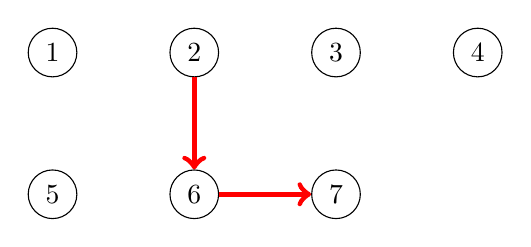
\begin{tikzpicture}[scale=0.9]
\node[draw, circle] (1) at (0,0) {1};
\node[draw, circle] (2) at (2,0) {2};
\node[draw, circle] (3) at (4,0) {3};
\node[draw, circle] (4) at (6,0) {4};
\node[draw, circle] (5) at (0,-2) {5};
\node[draw, circle] (6) at (2,-2) {6};
\node[draw, circle] (7) at (4,-2) {7};

\path[draw=red,thick,->,line width=2pt] (2) -- (6);
\path[draw=red,thick,->,line width=2pt] (6) -- (7);
\end{tikzpicture}
\end{center}

یافتن پوشش مسیر عمومی کمینه
تقریباً مشابه پوشش مسیر با راس‌های مجزا کمینه است.
تنها افزودن یال‌های تازه به گراف تطابق کافی است
به‌طوری که یال $a \rightarrow b$ همیشه برقرار باشد
هرگاه مسیری از $a$ به $b$ در گراف اولیه وجود دارد
(احتمالاً شامل چندین یال).

گراف تطابق برای گراف بالا بدین گونه است:
\begin{center}
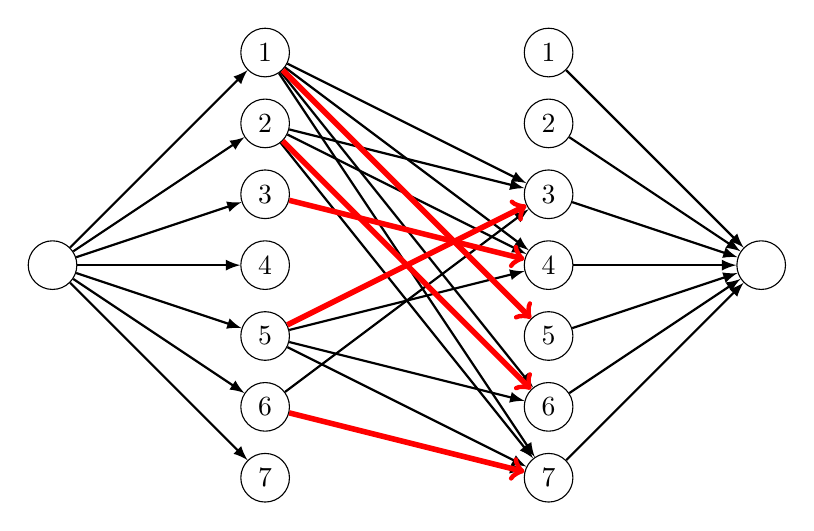
\begin{tikzpicture}[scale=0.9]
\node[draw, circle] (1a) at (0,6) {1};
\node[draw, circle] (2a) at (0,5) {2};
\node[draw, circle] (3a) at (0,4) {3};
\node[draw, circle] (4a) at (0,3) {4};
\node[draw, circle] (5a) at (0,2) {5};
\node[draw, circle] (6a) at (0,1) {6};
\node[draw, circle] (7a) at (0,0) {7};

\node[draw, circle] (1b) at (4,6) {1};
\node[draw, circle] (2b) at (4,5) {2};
\node[draw, circle] (3b) at (4,4) {3};
\node[draw, circle] (4b) at (4,3) {4};
\node[draw, circle] (5b) at (4,2) {5};
\node[draw, circle] (6b) at (4,1) {6};
\node[draw, circle] (7b) at (4,0) {7};

\node[draw, circle] (a) at (-3,3) {\phantom{0}};
\node[draw, circle] (b) at (7,3) {\phantom{0}};


%\path[draw,thick,->,>=latex] (1a) -- (5b);
\path[draw,thick,->,>=latex] (1a) -- (6b);
\path[draw,thick,->,>=latex] (1a) -- (7b);
\path[draw,thick,->,>=latex] (1a) -- (3b);
\path[draw,thick,->,>=latex] (1a) -- (4b);
\path[draw,thick,->,>=latex] (5a) -- (6b);
\path[draw,thick,->,>=latex] (5a) -- (7b);
%\path[draw,thick,->,>=latex] (5a) -- (3b);
\path[draw,thick,->,>=latex] (5a) -- (4b);
\path[draw,thick,->,>=latex] (6a) -- (7b);
%\path[draw,thick,->,>=latex] (6a) -- (7b);
\path[draw,thick,->,>=latex] (6a) -- (3b);
%\path[draw,thick,->,>=latex] (3a) -- (4b);
%\path[draw,thick,->,>=latex] (2a) -- (6b);
\path[draw,thick,->,>=latex] (2a) -- (7b);
\path[draw,thick,->,>=latex] (2a) -- (3b);
\path[draw,thick,->,>=latex] (2a) -- (4b);

\path[draw,thick,->,>=latex] (a) -- (1a);
\path[draw,thick,->,>=latex] (a) -- (2a);
\path[draw,thick,->,>=latex] (a) -- (3a);
\path[draw,thick,->,>=latex] (a) -- (4a);
\path[draw,thick,->,>=latex] (a) -- (5a);
\path[draw,thick,->,>=latex] (a) -- (6a);
\path[draw,thick,->,>=latex] (a) -- (7a);

\path[draw,thick,->,>=latex] (1b) -- (b);
\path[draw,thick,->,>=latex] (2b) -- (b);
\path[draw,thick,->,>=latex] (3b) -- (b);
\path[draw,thick,->,>=latex] (4b) -- (b);
\path[draw,thick,->,>=latex] (5b) -- (b);
\path[draw,thick,->,>=latex] (6b) -- (b);
\path[draw,thick,->,>=latex] (7b) -- (b);

\path[draw=red,thick,->,line width=2pt] (1a) -- (5b);
\path[draw=red,thick,->,line width=2pt] (5a) -- (3b);
\path[draw=red,thick,->,line width=2pt] (3a) -- (4b);
\path[draw=red,thick,->,line width=2pt] (2a) -- (6b);
\path[draw=red,thick,->,line width=2pt] (6a) -- (7b);


% \path[draw=red,thick,->,line width=2pt] (1a) -- (6b);
% \path[draw=red,thick,->,line width=2pt] (1a) -- (7b);
% \path[draw=red,thick,->,line width=2pt] (1a) -- (3b);
% \path[draw=red,thick,->,line width=2pt] (1a) -- (4b);
% \path[draw=red,thick,->,line width=2pt] (5a) -- (6b);
% \path[draw=red,thick,->,line width=2pt] (5a) -- (7b);
% \path[draw=red,thick,->,line width=2pt] (5a) -- (3b);
% \path[draw=red,thick,->,line width=2pt] (5a) -- (4b);
% \path[draw=red,thick,->,line width=2pt] (6a) -- (7b);
% \path[draw=red,thick,->,line width=2pt] (6a) -- (7b);
% \path[draw=red,thick,->,line width=2pt] (6a) -- (3b);
% \path[draw=red,thick,->,line width=2pt] (3a) -- (4b);
% \path[draw=red,thick,->,line width=2pt] (2a) -- (6b);
% \path[draw=red,thick,->,line width=2pt] (2a) -- (7b);
% \path[draw=red,thick,->,line width=2pt] (2a) -- (3b);
% \path[draw=red,thick,->,line width=2pt] (2a) -- (4b);

\end{tikzpicture}
\end{center}

\subsubsection{قضیه دیلوورث}

\index{قضیه دیلوورث}
\index{پادزنجیر}

یک \key{پادزنجیر} مجموعه‌ای از راس‌های گراف است
به‌طوری که هیچ مسیری بین هیچ دو راسی
با استفاده از یال‌های گراف وجود نداشته باشد.
\key{قضیه دیلوورث} بیان می‌کند
در یک گراف جهت‌دار بدون دور، اندازه
حداقل پوشش مسیری عمومی
برابر اندازه حداکثر پادزنجیر است.

برای نمونه، راس‌های ۳ و ۷ یک پادزنجیر
در گراف زیر تشکیل می‌دهند:

\begin{center}
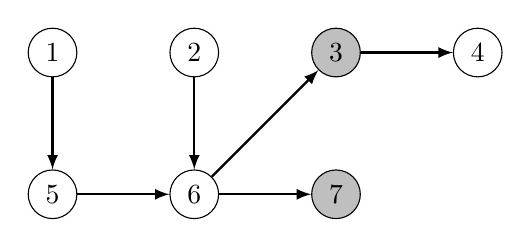
\begin{tikzpicture}[scale=0.9]
\node[draw, circle] (1) at (0,0) {1};
\node[draw, circle] (2) at (2,0) {2};
\node[draw, circle, fill=lightgray] (3) at (4,0) {3};
\node[draw, circle] (4) at (6,0) {4};
\node[draw, circle] (5) at (0,-2) {5};
\node[draw, circle] (6) at (2,-2) {6};
\node[draw, circle, fill=lightgray] (7) at (4,-2) {7};

\path[draw,thick,->,>=latex] (1) -- (5);
\path[draw,thick,->,>=latex] (2) -- (6);
\path[draw,thick,->,>=latex] (3) -- (4);
\path[draw,thick,->,>=latex] (5) -- (6);
\path[draw,thick,->,>=latex] (6) -- (3);
\path[draw,thick,->,>=latex] (6) -- (7);
\end{tikzpicture}
\end{center}

این یک پادزنجیر بیشینه است، زیرا ساخت هیچ پادزنجیری شامل سه رأس ممکن نیست. پیش‌تر دیدیم که اندازه یک پوشش مسیری عمومی کمینه برای این گراف برابر با دو مسیر است.